% !TEX root = 00_thesis.tex
% \chapter{Curriculum Vit\ae}
% \newpage

\pagestyle{empty}
\phantomsection\addcontentsline{toc}{chapter}{Curriculum Vit\ae}
% This Curriculum Vit\ae~is formatted following the suggested template of the \emph{Résumé for Researchers}, created by the Royal Society to support the evaluation of individuals’ varied contributions to research.%
% \footnote{\url{https://royalsociety.org/topics-policy/projects/research-culture/tools-for-support/resume-for-researchers/}}

\renewcommand{\arraystretch}{1.3}
\newcolumntype{P}[1]{>{\raggedright\arraybackslash}p{#1}}


\begin{minipage}{0.5\linewidth}
\begin{tabular}{@{}l}
  {\larger[2]Romain Jacob} \\
  % Doctoral Student -- 
  Open Science Enthusiast\\[10pt]
  born in Dec. 1990, French\\
  \href{http://www.romainjacob.net/}{www.romainjacob.net}
\end{tabular}
\end{minipage}%
\begin{minipage}{0.5\linewidth}
  \vspace{0pt}
  \raggedleft
  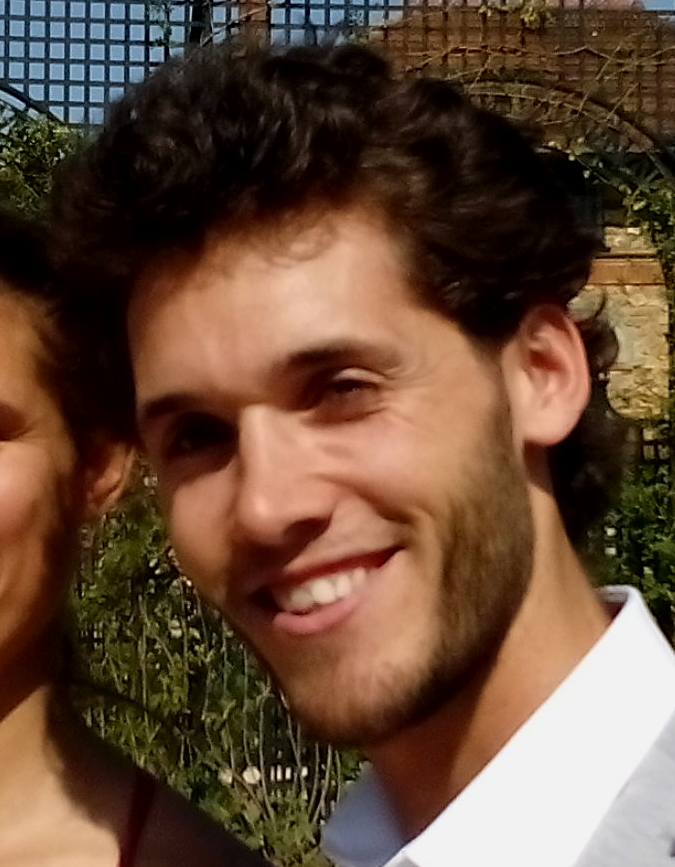
\includegraphics[width=3cm]{portrait_2018}
\end{minipage}%

% \paragraph{Key qualifications}
\begin{tabular}{@{}P{2.3cm}l@{}}
\cvbox &
  \textbf{Main qualifications}\\
  &Low-power Wireless Communication\\
  &Embedded and Cyber-Physical Systems\\
  &Real-time Scheduling\\
  &Formal Methods\\
\end{tabular}

% Education
\begin{tabular}{@{}P{2.3cm}P{10.5cm}}
\cvbox &
  \textbf{Education}\\
2015--2019 &
  Doctoral Studies in Computer Science \linebreak
  Supervised by Prof.\,Lothar Thiele \linebreak
  ETH Zurich, Switzerland \\
2011--2014 &
  Master in Engineering of Complex Systems \linebreak
  Advised by Prof.\,Jean-Jacques Lesage\linebreak
  % High Honors - Ranked 1 \linebreak
  École Normale Superieure (ENS) de Cachan, France\\
2012--2013 &
  Agrégation in Industrial Science -- Mechanics major \linebreak
  {\smaller[0.5] \emph{French exam for higher education teachers}}
  %\linebreak Passed – Ranked 1
  \\
% 2012-2013  &
~  &
  Master in Faculty Training for Higher Education\linebreak
  École Normale Superieure (ENS) de Cachan, France
  % \linebreak Honors
  \\
2010--2011 &
  Bachelor in Mechanical Engineering \linebreak
  Université Pierre et Marie Curie (UPMC, Paris 6), France
\end{tabular}

% \paragraph{Relevant positions}
\begin{tabular}{@{}P{2.3cm}P{10.5cm}}
\cvbox &
  \textbf{Experience}\\
2015--2019 &
  Doctoral Student and Scientific Assistant  \linebreak
  Computer Engineering and Networks Laboratory \linebreak
  Headed by Prof.\,Lothar Thiele\linebreak
  ETH Zurich, Switzerland \\
2013--2014 &
  Visiting Scholar \linebreak
  Vehicle Dynamics and Control laboratory \linebreak
  Headed by Prof.\,Karl Hedrick$^{\dag}$ \linebreak
  University of California (UC) Berkeley, CA, USA\\
\end{tabular}

\subsection*{How have you contributed to the generation of knowledge?}
% This module can be used to explain how you have contributed to the generation of new ideas and hypotheses and which key skills you have used to develop ideas and test hypotheses. It can be used to highlight how you have communicated on your ideas and research results, both written and verbally, the funding you have won and any awards that you have received. It can include a small selection of outputs, with a description of why they are of particular relevance and why they are considered in the context of knowledge generation. Outputs can include open data sets, software, publications, commercial, entrepreneurial or industrial products, clinical practice developments, educational products, policy publications, evidence synthesis pieces and conference publications that you have generated. Where outputs have a DOI please only include this.

\squarepar{%
  I led the development of \baloo,%
  \footnote{\href{http://www.romainjacob.net/baloo}{romainjacob.net/baloo}}
  a tool that assists embedded and cyber-physical system practitioners to leverage \emph{synchronous transmissions} --~a reliable low-power wireless technology.
  \baloo helps researchers explore the potential of synchronous transmissions for new applications domains and contexts.%
}

\squarepar
{%
  Using synchronous transmissions, I designed two wireless cyber-physical systems which provide real-time guarantees for distributed applications. These systems have been implemented and are openly available.%
  \footnote{\href{http://www.romainjacob.net/ttw}{romainjacob.net/ttw} -- \href{http://www.romainjacob.net/drp}{romainjacob.net/drp}}
  %
  The Time-Triggered Wireless design has been used to demonstrate the first-ever remote closed-loop control of multiple inverted pendulums over a multi-hop wireless network. This work received the ICCPS Best Paper%
  \footnote{\href{https://doi.org/10.1145/3302509.3311046}{10.1145/3302509.3311046}}
  and IPSN Best Demo%
  \footnote{\href{https://doi.org/10.1145/3302506.3312483}{10.1145/3302506.3312483}}
  awards in 2019.%
}

Furthermore, I worked on improving the reproducibility in networking experiments, which is challenged by the inherent variability of the experimental conditions.
I explored the statistics literature to identify the proper approaches and used these to define a concrete and rationale methodology for the design and analysis of experiments. This methodology has been implemented in a framework called \triscale,%
\footnote{\href{https://doi.org/10.5281/zenodo.3464274}{10.5281/zenodo.3464274}}
%
which is openly available for the different networking communities to use, extend, and build upon.%
\footnote{\href{https://doi.org/10.5281/zenodo.3451417}{10.5281/zenodo.3451417}}

\subsection*{How have you contributed to the development of individuals?}
% This module can be used to highlight expertise you provided which was critical to the success of a team or team members including project management, collaborative contributions, and team support. It can include your teaching activities, workshops or summer schools in which you were involved (for undergrads, grads and post-grads as well as junior colleagues), and the supervision of students and colleagues. It can be used to mention mentoring of members in your field and support you provided to the advancement of colleagues, be it junior or senior. It can be used to highlight the establishment of collaborations, from institutional (maybe interdisciplinary) to international. It can be used to describe where you exerted strategic leadership, how you shaped the direction of a team, organisation, company or institution.

\squarepar{%
  During my time at ETH Zurich, I have been teaching assistant in the \emph{Embedded Systems}, \emph{Low-Power System Design}, and \emph{Discrete Event Systems} lectures. Several students from these lectures carried on conducting a semester or master thesis under my supervision, resulting in 11 projects supervised so far.%
  \footnote{\href{http://www.romainjacob.net/students}{romainjacob.net/students}}%
}

\squarepar{%
  In 2014, I served as a contractual lecturer at the Institute of Technology of Tremblay-en-France (France), where I was responsible of a second year university-level Mechanics course on kinematics, kinetics, and dynamics.%
}

\pagebreak

\subsection*{How have you contributed to the wider research community?}
% This module can include various activities you have engaged in to progress the research community. It can be used to mention commitments including editing, reviewing, refereeing, committee work and your contributions to the evaluation of researchers and research projects. It can be used to mention the organisation of events that have benefited your research community. It can highlight contributions to increasing research integrity, and improving research culture (gender equality, diversity, mobility of researchers, reward and recognition of researchers’ various activities). It can be used to mention appointments to positions of responsibility such as committee membership and corporate roles within your department, institution or organisation, and recognition by invitation within your sector.

\squarepar{%
  During my doctoral studies, I have been heavily involved in IoTBench, a community-driven effort aiming to establish benchmarks for low-power wireless communication.%
  \footnote{\href{https://www.iotbench.ethz.ch/}{iotbench.ethz.ch}}
  %
  I participated in the organization of two conference workshops%
  \footnote{%
  \href{https://cpsbench2018.ethz.ch/}{cpsbench2018.ethz.ch} --
  \href{https://cps-iotbench2019.ethz.ch/}{cps-iotbench2019.ethz.ch}}
  %
  where I presented the vision and goals of IoTBench.%
  \footnote{\href{https://doi.org/10.3929/ethz-b-000339242}{10.3929/ethz-b-000339242}}%
}

I published tools to collect link quality measurements in low-power networks.%
\footnote{\href{https://doi.org/10.5281/zenodo.3354717}{10.5281/zenodo.3354717}}

\subsection*{How have you contributed to broader society?}
% This module can include examples of societal engagement and knowledge exchange. It can include engagement with industry and the private sector. It can be used to mention engagement with the public sector, clients and the broader public. It can be used to highlight positive stakeholder feedback, inclusion of patients in processes and clinical trials, and other impacts across research, policy, practice and business. It can be used to mention efforts to collaborate with particular societal or patient groups. It can be used to highlight efforts to advise policy-makers at local, national or international level and provide information through the press and on social media.

\squarepar
{%
  I try to communicate about my research to a wide audience, which I consider being a part of my job. Thus, I have taken part in various science communication activities, such as producing short videos and giving 3-minutes talks.%
  \footnote{\href{https://www.romainjacob.net/science-communication/}{romainjacob.net/science-communication}}%
}

% \squarepar
{%
  At ETH Zurich, I actively contributed to the representation of the scientific staff:
  in 2016, I directed a survey on the supervision of doctoral students%
  \footnote{\href{https://doi.org/10.3929/ethz-b-000262661}{10.3929/ethz-b-000262661}}
  %
  which highlighted some systematic issues, triggered many discussions and actions taken by ETH, and resulted in a revision of the doctoral studies regulations (currently ongoing).
  Since 2017, I co-preside VMITET, the association of the scientific staff in my department,%
  \footnote{\href{https://www.vmitet.ethz.ch/}{vmitet.ethz.ch}}
  %
  where I have been actively involved in representation activities towards the department management.%
}

\subsection*{Personal statement}
% Provide a personal statement that reflects on your overarching goals and motivation for the activities in which you have been involved.

\squarepar
{%
  I strongly believe in the principles generally known as ``Open Science''. In my work, this implies \eg favoring open and free software over commercial tools and submitting to open access conferences.
  Moreover, I try to systematically release data and code with all publications, aiming to make any plot or experiment reproducible by others, which I believe should be a standard in science.%
}

\squarepar{%
  Recently, I wrote down my own objectives and expectations regarding the way I intend to do research; this has materialized into a ``Pledge to Open Science'' which is publicly available on my personal website.%
  \footnote{\href{http://www.romainjacob.net/pledge-to-open-science/}{romainjacob.net/pledge-to-open-science}}
  %
  I will do my best to live and work by this principles, because I believe this is the right thing to do.%
}


% \subsection*{Additions}
% Mention career breaks, secondments, volunteering, part-time work and other relevant experience (including in time spent in different sectors) that might have affected your progression as a researcher.
